\documentclass[english,screen,twoside]{noahnotes}

\addbibresource{../references/references.bib}

\newcommand{\mathlabel}[1]{%
  \mathchoice
    {\mbox{#1}}%
    {\mbox{#1}}%
    {\mbox{\scriptsize #1}}%
    {\mbox{\tiny #1}}%
}

\usepackage{makecell}
\usepackage{multirow}

\title{Varmetransmission}
\date{\today}

\documentsetup{
  course={Varmetransmission},
  course-code={290221U002},
  course-short={Varmetransmission},
  instructor={Pourya Forooghi \& Mugisa Y. Kano},
  semester={Semester 5},
  toc-depth=2
}

\begin{document}

\frontmatter

\maketitle
\tableofcontents

\mainmatter

% WORKFLOW:LECTURES-BEGIN
% !TeX root = ../master.tex

\lecture{1}{2026-08-25}{Introduction to Heat Transfer}
These are the notes for the obligatory Heat Transfer course on the 5th semester of the Bs.c. in Mechanical Engineering at Aarhus University taught by Pourya Forooghi and Mugisa Y. Kano.

\section{Introduction to Heat Transfer}
Heat transfer as a subject has already been treated in the \href{https://www.bigum.dev/notes/partial-differential-equations.pdf}{Partial Differential Equations Course}.
Further, a related subject, namely \href{https://www.bigum.dev/notes/thermodynamics.pdf}{Thermodynamics} has also been studied.
However, whereas Thermodynamics mainly concerns itself with questions such as what the eventual equilibrium temperature will be or the total amount of heat transferred, heat transfer as a subject is more interested in questions such as the time it takes or the rate of heat transfer.

Heat Transfer is used in both power generation, heating/cooling/refrigeration, the chemical industry, indoor climate, thermal management and much more.
Further, new technology means heat transfer will remain very useful into the future as data centers, electronics, and turbine blades all need to meet higher cooling standards to maintain performance. 

Before we start, a quick note on terminology is useful.
We distinguish between \textit{Heat}, \textit{Heat transfer rate}, and \textit{Heat flux}.
Heat, $Q [\unit{\J}]$, denotes the amount of heat transfered.
The heat transfer rate, $\dot{Q}, [\unit{\J\per\s}]$, denotes the heat $Q$ transferred per unit time.
And finally, Heat flux, $\dot{q} [\unit{\W\per\m\squared}]$, is the heat transfer rate $\dot{Q}$ per unit area.

\subsection{Thermodynamics Recap}
Here will be given a short Introduction to the most important concepts of Thermodynamics which we will be dealing with here.
For a more in-depth review of the material see \href{https://www.bigum.dev/notes/thermodynamics.pdf}{my notes on the subject}.

The change in internal energy $u$ and enthalpy $h=u+p / \rho$ with temperature is generally given as:
\begin{itemize}
  \item Ideal Gasses:
    \begin{align*}
      \mathrm{d}u &= c_v \, \mathrm{d}T \\
      \mathrm{d}h &= c_p \, \mathrm{d}T
    .\end{align*}
  \item Incompressible substances:
    \begin{equation*}
      \mathrm{d}u = c \, \mathrm{d}T \quad (c \approx c_p \approx c_v)
    .\end{equation*}
\end{itemize}

Also, the 1st law of thermodynamics (the energy balance) states that the net energy transfer by heat, work, and mass from a system equals the change in the total energy of said system.
This also implies that the rate of energy transfer equals the rate of change in total energy.

\section{Heat Transfer Mechanisms}
We mainly work with three different heat transfer mechanisms.
These are \textit{Conduction}, \textit{Convection}, and \textit{Radiation}.

\subsection{Conduction} \label{sec:condintroduction}

\begin{wrapfigure}{r}{0.4\textwidth}
  \vspace{-1.5cm}
  \centering
  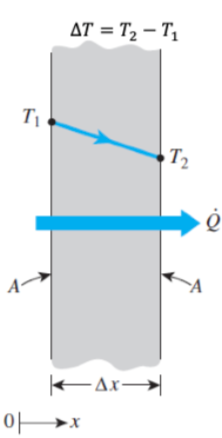
\includegraphics[width=\linewidth]{./figures/conduction.png}
  \caption{Cross section of a material displaying thermal conduction. Reproduced from \citepage{cengel2015heatmasstransfer}{fig.~1--23}.}
  \label{fig:conduction}
\end{wrapfigure}
Conduction is the transfer of energy from more energetic particles of a substance to the adjacent less energetic ones.
This happens in both solids and fluids, but always through a material medium, so it cannot happen in a vacuum.

The rate of conduction $\dot{Q}_{\mathrm{cond}}$ is generally given on a form resembling:
\begin{equation*}
  \dot{Q}_{\mathrm{cond}} \propto A \frac{\Delta T}{\Delta x}
\end{equation*}
where $A$ is the conducting area, $\Delta T$ is the change in temperature and $\Delta x$is the thickness of the cross-section.
This can be qualified by including the \textit{thermal conductivity} $k = \left[ \unit{\W\per\m\per\K} \right]$ which gives:
\begin{equation*}
  \dot{Q}_{\mathrm{cond}} = -k A \frac{\Delta T}{\Delta x}
.\end{equation*}
As $\Delta x \to 0$ this turns into \textit{Fourier's law of conduction (1D)}, given as:
\begin{equation} \label{eq:fourierlawconduction}
  \dot{q}_{\mathrm{cond}} = -k \frac{\mathrm{d}T}{\mathrm{d}x} 
\end{equation}
or in general vector form as 
\begin{equation*}
  \Vec{\dot{q}} = -k \nabla T
.\end{equation*}
The thermal conductivity varies with temperature.

We also define the \textit{thermal diffusivity} $\alpha$ as
\begin{equation*}
  \alpha = \frac{k}{\rho c_p}
.\end{equation*}
Roughly speaking, the thermal diffusivity determines how fast heat diffuses in a certain solid material.

\subsection{Convection}
\begin{wrapfigure}{r}{0.35\textwidth}
  \vspace{-1.5cm}
  \centering
  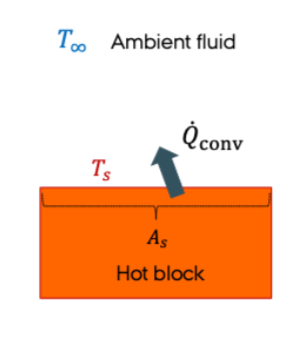
\includegraphics[width=\linewidth]{./figures/convection.png}
  \caption{Cross section of a material displaying convection.}
  \label{fig:convection}
\end{wrapfigure}
Convection is the transfer of energy as a result of bulk motion of fluid.
This always happens between a solid surface and a flowing fluid.
This can be both \textit{natural (free) convection}, i.e. flow created by bouyancy force and \textit{forced convection}, i.e. flow created by an external driving force.
When a material undergoes convection it will generally also be undergoing convection to some degree. 

The convection rate $\dot{Q}_{\mathrm{conv}}$ is normally given in a form such as
\begin{equation*}
  \dot{Q}_{conv} = \propto A_s (T_s - T_{\infty})
\end{equation*}
where $T_{\infty}$ is the far field temperature (or some other reference temperature), $T_s$ is the surface temperature, and $A_s$ is the heat transfer surface area. 
By introducing the heat transfer coefficient $h \left[ \unit{\W\per\m\squared\per\K}  \right]$ we arrive at Newton's law of cooling:
\begin{equation} \label{eq:newtoncool}
  \dot{Q}_{\mathrm{conv}} = h A_s \left( T_s - T_{\infty} \right)
.\end{equation}
It is important to remember the difference between the thermal conductivity $k$ and the heat transfer coefficient $h$.
Whereas the thermal conductivity is a material property the heat transfer coefficient is a property of the specific flow and must therefore be experimentally determined in all but the simplest cases.

\subsection{Radiation}
Thermal radiation is energy emitted by matter in form of electromagnetic waves.
Here, there is no need for an intervening medium, so this may also happen in a vacuum.
All bodies at a temperature above \qty{0}{\K} emit thermal radiation.
In general, radiation is a volumetric phenomenon but for opaque solids it is usually considered a surface phenomenon.
The heat transfer rate due to radiation, $\dot{Q}_{\mathrm{emit}}$:
\begin{equation*}
  \dot{Q}_{\mathrm{emit}} \propto A_s T_s^{4}
.\end{equation*}
For a black body (an ideal radiator) this is preciselu:
\begin{equation*}
  \dot{Q}_{\mathrm{emit}} = \sigma A_s T_s^{4}
\end{equation*}
where $\sigma = \qty{5,670e-8}{\W\per\m\squared\per\K^{4}}$ is Boltzmann's constant. The above is also known as Boltzmann's law.
For an arbitrary surface we instead have
\begin{equation*}
  \dot{Q}_{\mathrm{emit}} = \epsilon \sigma A_s T_s^{4}
\end{equation*}
where $0 \leq \epsilon \leq 1$ is the emissivity. 

Emissivity $\epsilon$ is a property of the radiating surface, which in reality varies with temperature but also depends on the wavelength of the electromagnetic wave.
For simplicity, we often use its mean value.

The opposite case of emitted radiation is that of absorbed radiation given by
\begin{equation*}
  \dot{Q}_{\mathrm{abs}} = \alpha \dot{Q}_{\mathrm{incident}}
\end{equation*}
where $0 \leq \alpha \leq 1$ is the absorptivity. 
Kirchoff's law of radiation states that at the same temperature and wavelength $\epsilon = \alpha$.

The net radiation heat transfer of a solid surface is
\begin{equation*}
  \dot{Q}_{\mathrm{rad}} = \dot{Q}_{\mathrm{emit}} - \dot{Q}_{abs}
.\end{equation*}
We have an important special case of the above for a surface entirely enclosed by a much larger surrounding surface as shown on \Cref{fig:radiation}, where
\begin{equation*}
  \dot{Q}_{\mathrm{rad}} = \epsilon \sigma A_s \left( T_s^{4} - T^{4}_{\mathrm{surr}} \right)
.\end{equation*}


\begin{figure} [ht]
  \centering
  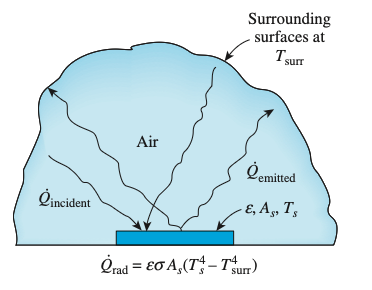
\includegraphics[width=0.4\linewidth]{./figures/radiation.png}
  \caption{Radiation between enclosed and enclosing body. Reproduced from \citepage{cengel2015heatmasstransfer}{fig.~1--40}.}
  \label{fig:radiation}
\end{figure}

% !TeX root = ../master.tex

\lecture{2}{2026-09-01}{Conduction, Pt. I}

\section{Conduction} \label{sec:conduction}
Heat transfer has both a \textit{direction} and a \textit{magnitude} and is therefore a vector quantity.
The magnitude in a specified direction is proportional to the \textit{temperature gradient}.
Heat conduction in a medium is \textit{steady}, when the temperature $T = T(x,y,z)$ does not vary with time and \textit{unsteady} or \textit{transient} when $T =(x,y,z,t)$ varies with time.
During transient heat transfer, the temperature normally varies with time as well as position.
In the special case of variation with time but not with position, the temperature of the medium changes uniformly with time -- such systems are termed \textit{lumped systems}.
Many small objects can be analyzed as being lumped systems.

In \Cref{sec:condintroduction}, heat conduction was defined as the transfer of thermal energy from more energetic particles of a medium to the adjacent less energetic ones.
We generally employ a coordinate system such that heat transfer in the positive direction of a coordinate axis is positive and vice versa.

We previously introduced Fourier's law of heat conduction in \Mref{eq:fourierlawconduction},
\begin{equation*}
  \dot{Q}_{\text{cond}} = -kA \frac{\mathrm{d}T}{\mathrm{d}x} 
\end{equation*}
where $k$ is the \textit{thermal conductivity} and $\frac{\mathrm{d}T}{\mathrm{d}x} $ is the temperature gradient.
In general the thermal conductivity of a material $k$ varies with time, however for most purposes an average value can be used for sufficiently accurate results.

Heat may also be generated throughout a medium.
E.g. the temperature of a resistor rises volumetrically when a current is applied.
Often it is also convenient to model the absorption of radiation such as solar energy or gamma rays as heat generation when those rays penetrate deep into a medium while being absorbed gradually such as for solar rays in a body of water.
For opaque bodies almost all absorption occurs within the first few microns of the surface, so in these cases the solar energy can be treated as heat flux on the surface. 
As heat generation is volumetric, it is usually specified per unit volume and denoted by $\dot{e}_{\text{gen}} = \left[ \unit{\W\per\m\cubed} \right]$.
The rate of heat generation may very with time as well as position.
When the variation w.r.t. the position is known, the total rate of heat generation in a medium of volume $\mathscr{V}$ can be determined from
\begin{equation} \label{eq:heatgenint}
  \dot{E}_{\text{gen}} = \int_{\mathscr{V}} \dot{e}_{\text{gen}} \, \mathrm{d}\mathscr{V}
.\end{equation}
In the special case of uniform heat generation \Mref{eq:heatgenint} reduces to
\begin{equation*}
  \dot{E}_{\text{gen}} = \dot{e}_{\text{gen}} \mathscr{V}
.\end{equation*}


\subsection{Heat Conduction Equation}
It is useful to expand \Mref{eq:fourierlawconduction} to more dimensions and include the internal heat generation.
In rectangular coordinates it can be shown that \Mref{eq:fourierlawconduction} can be written as
\begin{equation} \label{eq:heatcondcart}
  \frac{\partial }{\partial x} \left( k \frac{\partial T}{\partial x}  \right) + \frac{\partial }{\partial y} \left( k \frac{\partial T}{\partial y}  \right) + \frac{\partial }{\partial z} \left( k \frac{\partial T}{\partial z}  \right) + \dot{e}_{\text{gen}} = \rho c \frac{\partial T}{\partial t} 
.\end{equation}
for density $\rho$ and specific heat $c$.
In cylindrical coordinates it can be written
\begin{equation*}
  \frac{1}{r} \frac{\partial }{\partial r} \left( k r \frac{\partial T}{\partial r}  \right) + \frac{1}{r^2} \frac{\partial }{\partial \phi}  \left( k \frac{\partial T}{\partial \phi}  \right) + \frac{\partial }{\partial z} \left( k \frac{\partial T}{\partial z}  \right) + \dot{e}_{\text{gen}} = \rho c \frac{\partial T}{\partial t}
\end{equation*}
and in spherical coordinates it is
\begin{equation*}
  \frac{1}{r^2} \frac{\partial }{\partial r} \left( kr^2 \frac{\partial T}{\partial r}  \right) + \frac{1}{r^2 \sin^2 \theta} \frac{\partial }{\partial \phi} \left( k  \frac{\partial T}{\partial \phi} \right) + \frac{1}{r^2 \sin^2 \theta}\frac{\partial }{\partial \theta} \left( k \sin \theta \frac{\partial T}{\partial \theta}  \right) + \dot{e}_{\text{gen}} = \rho c \frac{\partial T}{\partial t} 
.\end{equation*}

\Mref{eq:heatcondcart} is the general heat conduction equation in rectangular coordinates.
In the case of constant thermal conductivity it reduces to:
\begin{equation} \label{eq:fourierbiot}
  \frac{\partial ^2 T}{\partial x^2}  + \frac{\partial ^2 T}{\partial y^2} + \frac{\partial ^2 T}{\partial z^2} + \frac{\dot{e}_{\text{gen}}}{k} = \nabla^2 T + \frac{\dot{e}_{\text{gen}}}{k} = \frac{1}{\alpha} \frac{\partial T}{\partial t}
\end{equation}
where $\alpha = k / \rho c$ is the \textit{thermal diffusivity of the material}.
\Mref{eq:fourierbiot} is known as the Fourier-Biot Equation.


\subsubsection{Special Cases of the Heat Equation}
For steady state systems the temperature does not vary with time $\frac{\partial T}{\partial t}  = 0$, so for steady-state:
\begin{equation} \label{eq:poisson}
  \frac{\partial ^2 T}{\partial x^2} + \frac{\partial ^2 T}{\partial y^2}  + \frac{\partial ^2 T}{\partial z^2} + \frac{\dot{e}_{\text{gen}}}{k} = \nabla^2 T + \frac{\dot{e}_{\text{gen}}}{k} = 0 
.\end{equation}
\Mref{eq:poisson} is known as the Poisson equation.

For transient systems with no heat generation \Mref{eq:fourierbiot} reduces to:
\begin{equation} \label{eq:diffusion}
  \frac{\partial ^2 T}{\partial x^2} + \frac{\partial ^2 T}{\partial y^2}  + \frac{\partial ^2 T}{\partial z^2} = \nabla^2 T = \frac{1}{\alpha} \frac{\partial T}{\partial t}
.\end{equation}
\Mref{eq:diffusion} is also known as the diffusion equation.

For steady-state systems without heat generation we arrive at \Mref{eq:laplace} also known as the Laplace equation:
\begin{equation*} \label{eq:laplace}
  \frac{\partial ^2 T}{\partial x^2}  + \frac{\partial ^2 T}{\partial y^2}  + \frac{\partial ^2 T}{\partial z^2} = \nabla ^2 T = 0
.\end{equation*}


\subsection{One-Dimensional Steady Heat Conduction}
We consider heat conduction through a large plane wall such as the wall of a house, the glass of a single pane window, or many other cases.
Heat conduction in these conditions can be approximated as being \textit{one-dimensional} since the conduction is dominant in one direction and negligible in the others.

\subsubsection{Plane Walls} \label{sec:planewall}
We consider a thin element of thickness $\Delta x$ in a large plane wall, as shown in \Mref{fig:condvolelement}.
We assume the density of the wall to be $\rho$, the specific heat to be $c$ and the area of
the wall normal to the direction of heat transfer to be $A$.

\begin{figure} [ht]
  \centering
  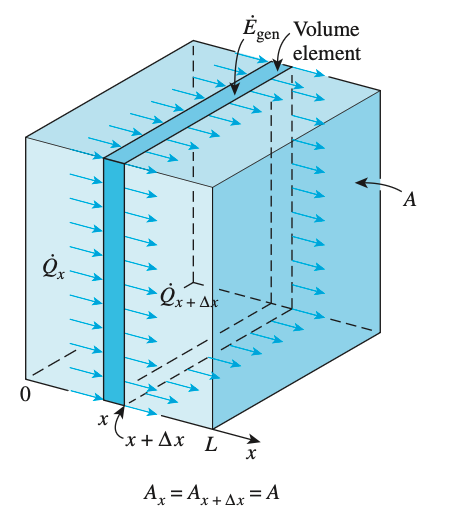
\includegraphics[width=0.4\linewidth]{./figures/condvolelement.png}
  \caption{One-dimensional heat conduction through a volume element in a large plane wall. Reproduced from \citepage{cengel2015heatmasstransfer}{fig 2--12}.}
  \label{fig:condvolelement}
\end{figure}

Taking the direction normal to the surface of the wall, i.e. through the plane on \Mref{fig:condvolelement} to be the $x$-direction we obtain:
\begin{align*}
  \frac{\mathrm{d}^2 T}{\mathrm{d}x^2} &= 0 \\
  \frac{\mathrm{d}T}{\mathrm{d}x} &= C_1 \\
  T &= C_1 x + C_2
.\end{align*}
On one side of the wall the temperature $T(0) = T_1$ and expressing the thickness of the wall as $L$ the boundary condition on the other side of the wall is $T(L) = T_2$ as shown on \Mref{fig:cond1dwall}

\begin{figure} [ht]
  \centering
  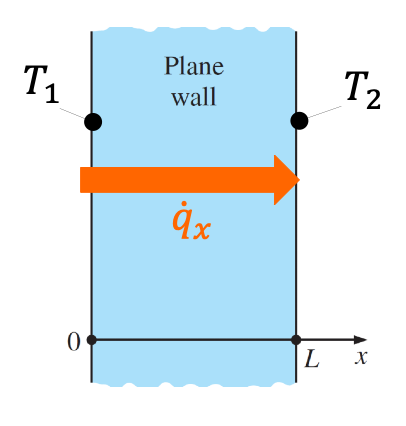
\includegraphics[width=0.4\linewidth]{./figures/cond1dwall.png}
  \caption{Conduction through a 1D-wall.}
  \label{fig:cond1dwall}
\end{figure}

As such
\begin{equation*}
  T(x) = T_1 + (T_2 - T_1) \frac{x}{L}
.\end{equation*}
This can then be used in \Mref{eq:fourierlawconduction} as
\begin{align*}
  \dot{q}_x &= -k \frac{\mathrm{d}T}{\mathrm{d}x}  \\
  \dot{q}_x(x) = \text{const.} &= k \frac{T_1 - T_2}{L} \\
  \dot{Q} &= k \frac{T_1 - T_2}{L}A 
.\end{align*}

\subsubsection{Cylindrical Geometries} \label{sec:cylgeo}
We consider a pipe of length $L$, inner and outer radiusses $r_1$ and $r_2$ and thermal conductivity $k$ as shown on \Mref{fig:f250}.

\begin{figure} [ht]
  \centering
  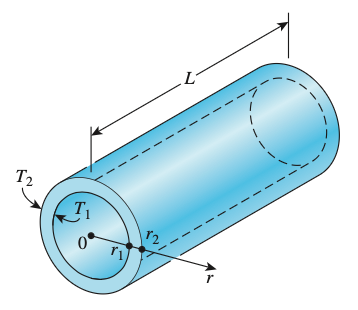
\includegraphics[width=0.4\linewidth]{./figures/f250.png}
  \caption{Schematic of a long cylinder with thickness $\Delta r = r_2 - r_1$. Reproduced from \citepage{cengel2015heatmasstransfer}{fig. 2--50}.}
  \label{fig:f250}
\end{figure}

The governing differential equation in this case is
\begin{equation*}
  \frac{\mathrm{d}}{\mathrm{d}r} \left( r \frac{\mathrm{d}T}{\mathrm{d}r}  \right) = 0 
\end{equation*}
with boundary conditions $T(r_1) = T_1, T(r_2) = T_2$.
Integrating the differential equation with respect to $r$ gives
\begin{gather*}
  r \frac{\mathrm{d}T}{\mathrm{d}r} = C_1  \frac{\mathrm{d}T}{\mathrm{d}r} = \frac{C_1}{r} \\
     T(r) = C_1 \ln r + C_2 
.\end{gather*}
Applying the boundary conditions this becomes
\begin{equation*}
  T(r) = T_1 + \left( T_2 - T_1 \right) \frac{\ln (r / r_1)}{\ln (r_2 / r_1)}
.\end{equation*}
This can be used in \Mref{eq:fourierlawconduction} as
\begin{gather*}
  \dot{q}_r (r) = -k \frac{\mathrm{d}T}{\mathrm{d}r} = k \frac{T_1-T_2}{\ln (r_2 /r_1) r} \\
  \dot{Q} = 2 \pi l k \frac{T_1 - T_2}{\ln (r_2 / r_1)}
.\end{gather*}


\subsubsection{Internal Heat Generation}
We now consider a long cylinder/wire which generates heat uniformly as shown on \Mref{fig:uniforminternalheatcyl}.
From steady state on cylindrical coordinates with uniform internal heat generatio we have
\begin{align*}
  \frac{1}{r}\frac{\mathrm{d}}{\mathrm{d}r} \left( r \frac{\mathrm{d}T}{\mathrm{d}r}  \right) + \frac{\dot{e}_{\text{gen}}}{k} &= 0 \\
  \frac{\mathrm{d}}{\mathrm{d}r} \left( r \frac{\mathrm{d}T}{\mathrm{d}r}  \right) &= - \frac{\dot{e}_{\text{gen}}}{k}r \\
  r \frac{\mathrm{d}T}{\mathrm{d}r} &= - \frac{\dot{e}_{\text{gen}}}{k} \frac{r^2}{2} + C_1 
.\end{align*}

\begin{figure} [ht]
  \centering
  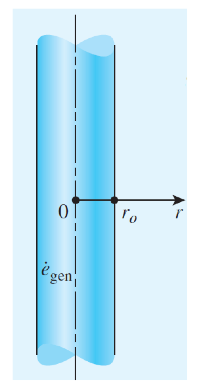
\includegraphics[width=0.25\linewidth]{./figures/uniforminternalheatcyl.png}
  \caption{Cylinder/wire conducting heat with uniform internal heat generation.}
  \label{fig:uniforminternalheatcyl}
\end{figure}

Due to symmetry we have a boundary condition at $r = 0$ as
\begin{align*}
  \frac{\mathrm{d}T}{\mathrm{d}r} (r=0) &= 0 \qquad \implies \qquad C_1 = 0 \\
  \frac{\mathrm{d}T}{\mathrm{d}r} &= - \frac{\dot{e}_{\text{gen}}}{k} \frac{r}{2} \\
  T &= - \frac{\dot{e}_{\text{gen}}}{k} \frac{r^2}{4} + C_2
.\end{align*}
Our second boundary condition is that the temperature at the edge is the surface temperature $T(r_0) = T_s$.
Hence
\begin{align*}
  T &= T_s + \frac{\dot{e}_{\text{gen}}}{4k} \left( r_0^2 - r^2 \right) \\
  T(r = 0) &= T_s + \frac{\dot{e}_{\text{gen}}}{4k} r_0^2
.\end{align*}

\subsection{Boundary Conditions}
A few different types of boundary conditions are normally employed
\begin{enumerate}
  \item Specified Temperature (Dirichlet)
  \item Specified heat flux (Neumann)
  \item Insulated boundary -- special case of Neumann with $\dot{q}_0 = 0$
  \item Thermal symmetry -- Symmetric temperature profile
  \item Convection (Robin / mixed) -- Specified convection from surfaces
\end{enumerate}

\subsection{Thermal Resistance}
Under steady conditions and surface temperatures the cumbersome differential equations can be avoided by instead introducing the concept of \textit{thermal resistivity} analogous to electrical resistivity.

\subsubsection{Conduction Resistance}
Analogous to electrical resistance:
\begin{equation*}
  I = \frac{V_1 - V_2}{R_e}
\end{equation*}
we now introduce thermal resistance
\begin{equation*}
  \dot{Q} = \frac{T_1 - T_2}{R}
.\end{equation*}
From the result for the conduction through a plane wall in \Mref{sec:planewall}
\begin{equation*}
  \dot{Q} = k \frac{T_1 - T_2}{L}A
\end{equation*}
the thermal resistivity can by comparison with the definition be read to equal
\begin{equation*}
  R_{\text{cond, wall}} = \frac{L}{kA}
.\end{equation*}
From the result for the conduction through a cylinder from \Mref{sec:cylgeo}
\begin{equation*}
  \dot{Q} = 2 \pi l k \frac{T_1 - T_2}{\ln (r_2/r_1)}
\end{equation*}
we see that the thermal resistivity here is
\begin{equation*}
  R_{\text{cond,cyl}} = \frac{\ln (r_2/r_1)}{2\pi l k}
.\end{equation*}

\subsubsection{Series Resistance Networks}
The above conduction resistances can be combined.
Say two walls are placed against each other.
Following the above the thermal conduction through each wall is
\begin{align*}
  \dot{Q}_{2} &= \frac{T_1 - T_2}{R_{\text{wall},1}} \\
  \dot{Q}_3 &= \frac{T_2 - T_3}{R_{\text{wall},2}}
.\end{align*}
We can then eliminate the intermediate temperature at the interface between the walls $T_2$ as
\begin{equation*}
  \dot{Q}_{23} = \frac{T_1 - T_3}{R_{\text{wall},1} + R_{\text{wall},2}}
.\end{equation*}
We define the convective thermal resistance as
\begin{equation*}
  \dot{Q} = h A \left( T_{\infty} - T_s \right)
.\end{equation*}
And as such for the case shown on \Mref{fig:seriesthermalres}
\begin{align*}
  \dot{Q}_{1} &= h_1 A \left( T_{\infty 1} - T_1 \right) = \frac{T_{\infty1} - T_1}{R_{\text{conv},1}}  \\
  \dot{Q}_{4} &= h_2 A \left( T_3 - T_{\infty 2} \right) = \frac{T_3 - T_{\infty 2}}{R_{\text{conv}, 2}}
.\end{align*}
These can then all be combined to yield the total conduction through the wall
\begin{equation*}
  \dot{Q} = \frac{T_{\infty 1} - T_{\infty 2}}{R_{\text{conv},1} + R_{\text{conv},2} + R_{\text{wall},1} + R_{\text{wall},2}}
.\end{equation*}


\begin{figure} [ht]
  \centering
  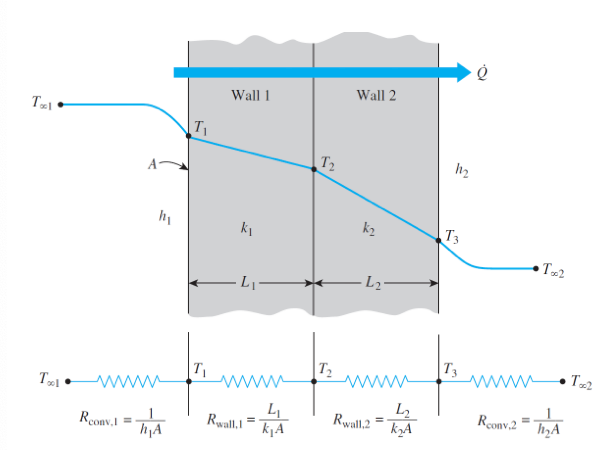
\includegraphics[width=0.7\linewidth]{./figures/seriesthermalres.png}
  \caption{Thermal resistance in series.}
  \label{fig:seriesthermalres}
\end{figure}

\subsubsection{Parallel and Generalized Resistance Networks}
Analogous to electrical resistances thermal resistances can also be in parallel as shown on \Mref{fig:parprob}.
In such cases the total resistance, $R_{\text{tot}}$ is calculated using the reciprocal of the reciprocal sums of the individual parallel resistances.
\begin{equation*}
  \frac{1}{R_{\text{tot}}} = \frac{1}{R_1} + \frac{1}{R_2}
.\end{equation*}

Parallel thermal resistances only occur in 2D or 3D whilst thermal resistance theory is based on 1D solutions so this is only an approximation.

\begin{figure} [ht]
  \centering
  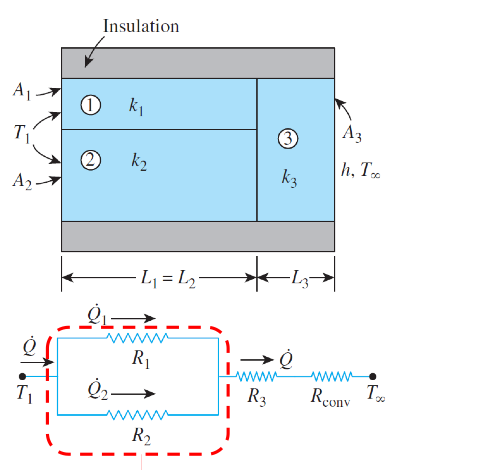
\includegraphics[width=0.5\linewidth]{./figures/parprob.png}
  \caption{Parallel thermal resistance}
  \label{fig:parprob}
\end{figure}

\subsubsection{Thermal Contact Resistance}
In the above, we assumed ``perfect contact'' at the interface between layers, and thus no temperature drop at the interface.
In reality no such interface exists and as a result any interface will contain imperfections and air gaps.
Thus, an interface offers some resistance to heat transfer which is characterised by a \textit{thermal contact resistance} $R_c$ for a unit interface area.
This can be expressed in a manner analogous to Newton's law of cooling
\begin{equation*}
  \dot{Q} = h_c A \Delta T_{\text{interface}}
\end{equation*}
where $A$ is the apparent interface area, $\Delta T_{\text{interface}}$ is the effective temperature difference at the interface and $h_c$ is the \textit{thermal contact conductance} defined as
\begin{equation*}
  h_c = \frac{\dot{Q}/A}{\Delta T_{\text{interface}}}
\end{equation*}
which is the inverse of thermal contact resistance $R_c$
\begin{equation*}
  R_c = \frac{1}{h_c} = \frac{\Delta T_{\text{interface}}}{\dot{Q}/A}
.\end{equation*}

It is also worth noting that the heat transfer rate is the quotient of the temperature difference over the interface $\Delta T_{\text{interface}}$ and the created thermal resistance $R_c / A$ as
\begin{equation*}
  \dot{Q} = \frac{\Delta T_{\text{interface}}}{R_c / A}
.\end{equation*}


% !TeX root = ../master.tex

\lecture{3}{2026-09-8}{Conduction, Pt. II}

\subsection{Steady Heat Conduction in 2D \& 3D}

\subsubsection{Analytical and Numerical Solutions}
For multidimensional steady conduction, the governing equation is the steady heat conduction equation,
\begin{equation*}
   \nabla^2 T + \frac{\dot e_\mathrm{gen}}{k}=0.
.\end{equation*}
Analytical solutions exist for relatively simple geometries and boundary conditions, but rapidly become cumbersome.
Practical multidimensional problems are therefore commonly solved numerically or by use of existing analytical solutions.
These existing analytical solution are often given in term of a shape factor $S [\unit{\m}]$.

\subsubsection{Conduction Shape Factors}
The shape factor is defined such, that the stationary heat flow:
\begin{align*}
  q''_x &= -k \frac{\partial T}{\partial x} \\
  q''_y &= -k \frac{\partial T}{\partial y} 
\end{align*}
can be written on a simple form:
\begin{equation} \label{eq:condshape}
  Q = S k \Delta T_{1-2}
.\end{equation}
Hence, the shape factors can only be used when considering conduction between two surfaces with constant temperature.
The conduction shape factors depend only on the \textit{geometry} of the system.
These conduction shape factors $S$ have been determined for a number of standard configurations and a small excerpt of these are shown in \citepage{cengel2015heatmasstransfer}{Table 3--7}.
These are also only applicable when the mode of heat transfer is conduction and they are therefore not useful for liquids or gasses.
By observation of \Mref{eq:condshape} it is evident that the conduction shape factor $S$ is related to thermal resistance $R$ by
\begin{equation*}
  R = \frac{1}{kS} \qquad \iff \qquad S = \frac{1}{kR}
.\end{equation*}


\subsection{Extended and Finned Surfaces}
As mentioned previously, the rate of heat transfer from a surface at temperature $T_s$ to the surrounding medium at temperature $T_{\infty}$ is per Newton's law of cooling, \Mref{eq:newtoncool}:
\begin{equation*}
  \dot{Q}_{\text{conv}} = h A_s \left( T_s - T_{\infty} \right)
.\end{equation*}
Hence, the heat transfer rate can be increased by either increasing the temperature difference, the convection heat transfer coefficient $h$ or the surface area $A_s$.
The temperature difference is often fixed by design constraints and increasing $h$ may require installing a pump or fan or replacing an existing one with a larger one, but this may also not always be practical.
The other alternative is increasing surface area by attaching \textit{extended surfaces} called \textit{fins} made of highly conductive material to the surface.
The addition of fins often increase the heat transfer from a surface severalfold.

\subsubsection{Fin Equation}
From an energy balance on a fin, using Fourier's law of heat conduction it can be shown that the differential equation governing heat transfer in fins is:
\begin{equation*}
  \frac{\mathrm{d}}{\mathrm{d}x} \left( k A_c \frac{\mathrm{d}T}{\mathrm{d}x}  \right) = h p \left( T - T_{\infty} \right)
.\end{equation*}
In general, the cross sectional area $A_c$ and the perimeter $p$ of a fin vary with $x$ which makes the above differential equation hard to solve.
For \textit{constant cross section} and \textit{constant thermal conductivity} the above reduces to:
\begin{equation*}
  \frac{\mathrm{d}^2 T}{\mathrm{d}x^2} = \frac{h p}{k A_c} \left( T - T_{\infty} \right)
.\end{equation*}
This can also be expressed as
\begin{equation} \label{eq:reducedfinm}
  \frac{\mathrm{d}^2 \theta}{\mathrm{d}x^2} = m^2 \theta
\end{equation}
where
\begin{equation*}
  m^2 = \frac{hp}{k A_c}
\end{equation*}
and $\theta = T - T_{\infty}$ is the \textit{temperature excess}.
As $m$ in \Mref{eq:reducedfinm} is assumed constant the differential equation can be solved yielding
\begin{equation*}
  \theta(x) = C_1 e^{mx} + C_2 e^{-mx}
\end{equation*}
where $C_1$ and $C_2$ are arbitrary constants whose values depend on the boundary conditions at the base and at the tip of the fin.

The temperature of the plate to which the fin is attached is normally known in advance.
Therefore, at the fin base we have a Dirichlet BC, expressed as
\begin{equation*}
  \theta(0) = \theta_b = T_b - T_{\infty}
.\end{equation*}
At the fin tip, however, we have several possibilities, which are explained in \Mref{sec:bc}.

\subsubsection{Boundary Conditions for Fins} \label{sec:bc}

\paragraph{Infinitely Long Fins}
For a sufficiently long fin of uniform cross section, the temperature of the fin at the fin tip $T(L)$ approaches the environment temperature $T_{\infty}$ and thus $\theta = T(L) - T_{\infty} \to 0$.
Therefore, for an infinitely long fin we have the boundary condition at the fin tip:
\begin{equation*}
  \theta(L) = T(L)- T_{\infty} = 0, \qquad L \to \infty
.\end{equation*}
In this case our general solution after applying BC's become:
\begin{equation*}
  \theta(x) = \theta_b e^{-m x} = \theta_b e^{-x \sqrt{\frac{h p}{k A_{c}}}}
.\end{equation*}
This corresponds to the temperature decreasing exponentially from $T_b$ to $T_{\infty}$.
The steady rate of heat transfer for an infinitely long fin can be determined from Fourier's law of heat conduction
\begin{equation*}
  \dot{Q}_{\text{long fin}} = - k A_{c} \frac{\mathrm{d}T}{\mathrm{d}x} \bigg|_{x = 0} = \sqrt{h p k A_c} \theta_b
\end{equation*}
where $p$ is the perimeter, $A_c$ is the cross-sectional area of the fin, and $x$ is the distance from the fin base.

\paragraph{Negligible Heat Loss from the Fin Tip}
Few fins are actually sufficiently long that their temperature approaches the surrounding temperature at the tip.
A more realistic expectation is for heat transfer from the fin tip to be negligible since the heat transfer is proportional to surface area and little of the total surface area is in the tip.
In such cases, the fin tip can be assumed adiabatic yielding the following boundary condition at the fin tip:
\begin{equation*}
  \frac{\mathrm{d}\theta}{\mathrm{d}x} \bigg|_{x = L} = 0
.\end{equation*}
After applying both BCs to the solution to the differential equation we get the following expression for the temperature excess along the fin:
\begin{equation*}
  \theta(x) = \theta_b \frac{\cosh m (L-x)}{\cosh m L}
\end{equation*}
and the rate of heat transfer can, again, be determined from Fourier's law of heat conduction:
\begin{equation*}
  \dot{Q}_{\text{adiabatic tip}} = - k A_c \frac{\mathrm{d}T}{\mathrm{d}x} \bigg|_{x = 0} = \sqrt{h p k A_c} \theta_b \tanh m L
.\end{equation*}

\paragraph{Specified Temperature}
Instead of assuming the fin tip does not transfer heat or that the fin is sufficiently long for the fin tip to reach the surrounding temperature, it is often more accurate to specify a temperature at the fin tip which is assumed to be fixed.
This temperature is often a bit higher than room temperature but the temperature excess at the tip under normal operating conditions must often be determined exponentially.
In this case, the boundary condition for the fin tip is
\begin{equation*}
  \theta(L) = \theta_L = T_L - T_{\infty}
.\end{equation*}
In this case the temperature distribution along the wing is described by
\begin{equation*}
  \theta(x) = \theta_b \frac{\left( \frac{\theta_L}{\theta_b} \right) \sinh m x + \sinh m (L-x)}{\sinh m L}
.\end{equation*}
From Fourier's law of heat condution, the rate of heat transfer from the fin in this case is
\begin{equation*}
  \dot{Q}_{\text{specified temperature}} = - k A_{c} \frac{\mathrm{d}T}{\mathrm{d}x} \bigg|_{x = 0} = \sqrt{h p k A_c} \theta_b \frac{\cosh m L - \frac{\theta_L}{\theta_b}}{\sinh m L}
.\end{equation*}

\paragraph{Convection from Fin Tip}
In actuality, fin tips are exposed to the surroundings, and thus the proper boundary conditions for the fin tip is convection that also may include the effects of radiation.
In this case, the boundary condition at the fin tip can be obtained from an energy balance at the fin tip ($\dot{Q}_{\text{cond}} = \dot{Q}_{\text{conv}}$.
This yields the boundary condition:
\begin{equation*}
  - k A_c \frac{\mathrm{d}T}{\mathrm{d}x} \bigg|_{x = L} = h A_c \theta_L
.\end{equation*}
In this case, the temperature profile across the fin is
\begin{equation*}
  \theta(x) = \theta_b \frac{\cosh m (L-x) + \left( \frac{h}{m k} \right) \sinh m (L-x)}{\cosh m L + \left( \frac{h}{m k} \right) \sinh m L}
.\end{equation*}
The rate of heat transfer here is
\begin{equation*}
\dot{Q}_{\text{convection}} = - k A_c \frac{\mathrm{d}T}{\mathrm{d}x} \bigg|_{x = 0} = \sqrt{h p k A_c } \theta_b \frac{\sinh m L + \frac{h}{m k} \cosh m L}{\cosh m L + \frac{h}{m k} \sinh m L}
.\end{equation*}

\subsubsection{Fin Efficiency}
We now consider the surface of a \textit{plane wall} at temperature $T_b$ exposed to a medium at temperature $T_{\infty}$.
Heat is lost from the surface to the surrounding medium by convection with a heat tranfer coefficient of $h$.
Disregarding radiation, heat transfer from a surface area $A_s$ is $\dot{Q} = h A_s (T_s - T_{\infty})$.

Now we attach a fin of constant cross sectional-area $A_c$ and length $L$ to the surface with perfect contact.
Now, heat is transferred from the surface to the fin by conduction and from the fin to the medium by convection with the same heat transfer coefficient $h$.
The temperature of the fin is $T_b$ at the base and gradually decreases toward the tip.
Convection from the fin causes the temperature to drop somewhat from the midsection toward the outer surface.
However, the cross-sectional area of the fin is usually very small and thus the temperature at any cross section can be assumed uniform.

In the limiting case of zero thermal resistance or infinite thermal conductivity, the temperature of the fin is uniform at the base at $T_b$.
The heat transfer from the fin is maximum in this case and can be expressed as
\begin{equation*}
  \dot{Q}_{\text{fin, max}}  = h A_{\text{fin}} (T_b - T_{\infty})
.\end{equation*}
In reality, the temperatyre of the fin drops along the fin and thus the heat transfer from the fin is less because of the decreasing temperature excess $T(x) - T_{\infty}$.
To account for this, we define fin efficiency as
\begin{equation*}
  \eta_{\text{fin}} = \frac{\dot{Q}_{\text{fin}}}{\dot{Q}_{\text{fin, max}}} = \frac{\text{actual heat transfer rate from the fin}}{\text{Heat transfer rate from the fin if the entire fin was at base temperature}}
.\end{equation*}

Hence, the total heat transfer from a finned surface is
\begin{equation*}
  \dot{Q}_{\text{fin}} = \eta_{\text{fin}} \underbracket{A_{\text{fin}} h \theta_b}_{\dot{Q}_{\text{fin max}}}
.\end{equation*}
And the total heat transfer is
\begin{align*}
  Q_{\text{total,fin}} &= \dot{Q}_{\text{fin}} + \dot{Q}_{\text{unfin}} \\
  &= \eta_{\text{fin}} A_{\text{fin}} h \theta_b + A_{\text{unfin}} h \theta_b \\
  &= \left( \eta_{\text{fin}} A_{\text{fin}} + A_{\text{unfin}} \right) h \theta_b
.\end{align*}

The fin efficiency in the cases of \textit{very long fins} and \textit{adiabatic tips} can be expressed as:
\begin{align*}
  \eta_{\text{ling fin}} &= \frac{1}{mL} \\
  \eta_{\text{adiabatic tip}} &= \frac{\tanh mL}{mL}
.\end{align*}


\subsubsection{Fin Effectiveness}
There is no assurance that adding fins to a surface will \textit{enhance} heat transfer.
The performance of the fins is judged on the basis of the enhancement in heat transfer relative to the \textit{no-fin} case.
The performance of fins is expressed in terms of the fin effectiveness $\epsilon_{\text{fin}}$:
\begin{equation*}
  \epsilon_{\text{fin}} = \frac{\dot{Q}_{\text{fin}}}{\dot{Q}_{\text{no fin}}} = \frac{\dot{Q}_{\text{fin}}}{h A_b \theta_b}
.\end{equation*}
Hence, $A_b$ is the cross sectional area of the fin at the base and $\dot{Q}_{\text{no fin}}$ represents the rate of heat transfer from this area if no fin were attached.
An effectiveness of $\epsilon_{\text{fin}} = 1$ indicates that the addiction of fins to the surface does not affect heat transfer at all.

The fin efficiency and fin effectiveness are different quantities but related to each other by:
\begin{equation*}
  \epsilon_{\text{fin}} = \frac{A_{\text{fin}}}{A_b} \theta_{\text{fin}}
.\end{equation*}

The overall effectiveness, $\epsilon_{\text{fin, overall}}$ is the effectiveness of the addition of fins to the entire area:
\begin{equation*}
  \epsilon_{\text{fin, overall}} = \frac{\dot{Q}_{\text{total, fin}}}{\dot{Q}_{\text{total, no fin}}} = \frac{\eta_{\text{fin}} A_{\text{fin}} + A_{\text{unfin}}}{A_b + A_{\text{unfin}}}
.\end{equation*}


% !TeX root = ../master.tex

\lecture{4}{2026-09-15}{Conduction, Pt. III}

\subsection{Transient Heat Conduction}
In transient heat conduction, the temperature field changes with time,
\begin{equation*}
  T = T(x,y,z,t).
.\end{equation*}
The governing heat equation therefore retains the transient term
\begin{equation*}
  \rho c \frac{\partial T}{\partial t}.
.\end{equation*}

\subsubsection{Lumped System Analysis}
In heat transfer analysis, some bodies are observed to behave like a ``lump'', i.e. whose interior temperature remains uniform at any point during a heat transfer process.
The temperature of such bodies can be taken to be a function of time only, $T(t)$.
Analysis utilizing this idealization is known as \textit{lumped system analysis}.
This is often applicable for small bodies.

We consider a body of arbitrary shape of mass $m$, volume $\mathscr{V}$, surface area $A_s$, density $\rho$, and specific heat $c_p$ initially at uniform temperature $T_i$.
At time $t = 0$, the body is placed into a medium at temperature $T_{\infty}$, and heat transfer takes place between the body and the medium with heat transfer coefficient $h$.
We assume the system to be lumped, such that the temperature within the body remains uniform, $T = T(t)$.
During a differential time element $\mathrm{d}t$, the temperature of the body rises by a differential amount $\mathrm{d}T$.
An energy balance of the solid for the time interval $\mathrm{d}t$ can be expressed as
\begin{equation*}
  h A_s \left( T_{\infty}-T \right) \, \mathrm{d}t  = m c_p \, \mathrm{d}T
.\end{equation*}
Noting that $m = \rho \mathscr{V}$ and $\mathrm{d}T = \mathrm{d}(T-T_{\infty})$ since $T_{\infty} = \text{constant}$ the above can be rearranged as
\begin{equation*}
  \frac{\mathrm{d}(T-T_{\infty})}{T-T_{\infty}} = - \frac{h A_s}{\rho \mathscr{V} c_p} \, \mathrm{d}t
.\end{equation*}
integrating from $t = 0$, at which $T = T_i$ to a time $t$ at which $T = T(t)$ gives
\begin{equation*}
  \ln \frac{T(t) - T_{\infty}}{T_i - T_{\infty}} = - \frac{h A_s}{\rho \mathscr{V}c_p}t
.\end{equation*}
Rearranging we obtain
\begin{equation} \label{eq:lumpedtemp}
  T - T_{\infty} = (T_i - T_{\infty}) e^{-bt}
\end{equation}
where
\begin{equation*}
  b = \frac{h A_s}{\rho \mathscr{V} c_p} \quad \unit{\per\s}
\end{equation*}
is a positive quantity.
The reciprocal of $b$, is termed $\tau$ and is called the time constant defined as:
\begin{equation*}
  \tau = \frac{1}{b} = \frac{\rho c_p \mathscr{V}}{h A_s} \qquad \implies \qquad \theta = e^{- \frac{t}{\tau}}
.\end{equation*}


\paragraph{Heat Transfer Rate and Total Heat Transfer}
Once the temperature $T(t)$ at time $t$ is found from \Mref{eq:lumpedtemp}, the rate of convection heat transfer between the body and its environment at that time can be determined from Newton's law of cooling as
\begin{equation*}
  \dot{Q}(t) = h A_s \left( T(t) - T_{\infty} \right)
.\end{equation*}
The \textit{total amount} of heat transfer between the body and the surrounding medium over the time interval $t = 0$ to $t$ is simply the change in the energy content of the body:
\begin{equation*}
  Q = m c_p (T(t) - T_i)
.\end{equation*}
The amount of heat transfer reaches its upper limit when the body reaches the surrounding temperature, therefore the \textit{maximum} heat transfer between the body and its surroundings is
\begin{equation*}
  Q_{\text{max}} = m c_p (T_{\infty} - T_i)
.\end{equation*}


\subsubsection{Biot Number and Lumped-System Criterion}
Now, we must determine when lumped analysis is appropriate to use.
The first step in establishing such a criterion is to define a characteristic length as:
\begin{equation*}
  L_c = \frac{\mathscr{V}}{A_s}
\end{equation*}
and a dimensionless \textit{Biot number} $\mathrm{Bi}$ as
\begin{equation} \label{eq:biot}
  \mathrm{Bi} = \frac{h L_c}{k}
.\end{equation}
The characteristic length $L_c$ to be used in the Biot number for simple geometries in which heat transfer is one-dimensional, such as a large plane wall of thickness $2L$, a long cylinder of radius $r_o$, and a sphere of radius $r_o$ becomes $L$, $r_o / 2$, and $r_o / 3$, respectively.
The Biot number is the ratio of internal resistance of a body to heat conduction to its external resistance to heat convection. 
Therefore a small Biot number represents a small resistance to conduction and thus small temperature gradients within the body.

Lumped system analysis assumes a uniform temperature distribution throughout the body.
Thus lumped system analysis is exact when $\mathrm{Bi} = 0$ and approximate when $\mathrm{Bi} > 0$.
It is generally accepted that lumped system analysis is applicable if
\begin{equation*}
  \mathrm{Bi} \leq \num{0,1} 
.\end{equation*}


\subsubsection{One-Dimensional Transient Heat Conduction}
We now move on to transient heat conduction in non-lumped bodies one-dimensional bodies.
We now consider the variation of temperature with \textit{time} and \textit{position} in one-dimensional problems such as those associated with a large plane wall, a long cylinder, and a sphere.

\paragraph{Transient Conduction in a Plane Wall}
We consider a wall of total thickness $2L$.
The $x$-coordinate is measured from the centre plane, so $x = 0$ is the middle and $x = L$ is the exposed face.
The same fluid is on both sides.

\begin{figure} [ht]
  \centering
  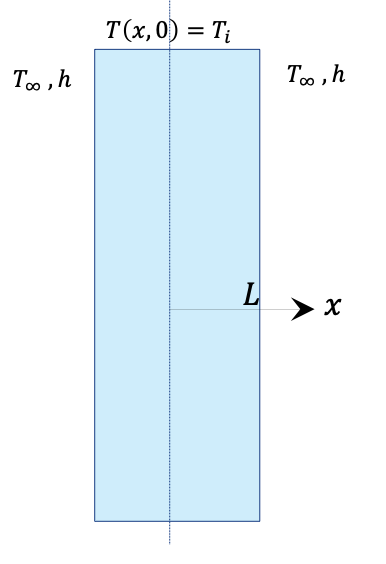
\includegraphics[width=0.4\linewidth]{./figures/transientwall.png}
  \caption{Transient Conduction in a Plane Wall.}
  \label{fig:transientwall}
\end{figure}

The left side at $x = 0$ is insulated (i.e. no heat leaves) and the right side $x = L$ loses heat to the environment through convection.
The initial state is everything starting at the same temperature.
Our governing differential equation is
\begin{equation*}
  \frac{\partial ^2 T}{\partial x^2}  = \frac{1}{\alpha} \frac{\partial T}{\partial t}, \qquad \alpha = \frac{k}{\rho c_p}
.\end{equation*}

\paragraph{Dimensionless Temperature, Biot Number and Fourier Number}
Solving the above equation with the given BC's and IC would give $T$ as a function of $x$, $t$, $T_i$, $T_{\text{inf}}$, $k$, $\alpha$, $h$ and $L$.
Instead, we can also opt to use dimensional analysis to make the problem dimension-less.
First, we define the dimensionless temperature:
\begin{equation*}
  \theta = \frac{T - T_{\infty}}{T_i - T_{\infty}}
\end{equation*}
this is the temperature excess.

We also define the Fourier number, $\mathrm{Fo}$:
\begin{equation*}
  \mathrm{Fo} = \frac{\alpha t}{L^2} = \frac{t}{L^2 / \alpha}
.\end{equation*}
The Fourier number can be seen as the ratio of elapsed time to the time required for heat to diffuse through the body.
So a small $\mathrm{Fo}$ means the process just started and a large $\mathrm{Fo}$ means diffusion has had a long time to act.

Using the Fourier and previously introduced Biot numbers the temperature excess of the wall can be written as:
\begin{equation*}
  \theta(x,t) = \frac{T - T_{\infty}}{T_i - T_{\infty}} = \underbracket{f_1 (\mathrm{Fo} \mathrm{Bi})}_{\text{Time part}} \cdot \underbracket{f_2 \left( \frac{x}{L}, \mathrm{Bi} \right)}_{\text{Position part}}
.\end{equation*}


\paragraph{One-Term Approximation}
The exact solution to the above is an infinite series.
For $\mathrm{Fo} > \num{0,2}$ is the first term of the series, however, normally enough.
Then:
\begin{align*}
  f_1(\mathrm{Fo}, \mathrm{Bi}) &\approx A_1 e^{-\lambda_1^2 \mathrm{Fo}} \\
  f_2 \left( \frac{x}{L}, \mathrm{Bi} \right) &\approx \cos \left( \lambda_1 \frac{x}{L} \right)
.\end{align*}
Meaning
\begin{equation*}
  \theta = \frac{T - T_{\infty}}{T_i - T_{\infty}} = A_1 e^{-\lambda_1^2 \cdot \mathrm{Fo}} \cdot \cos \left( \lambda_1 \frac{x}{L} \right)
\end{equation*}
where, $A_1$ and $\lambda_1$ are functions of $\mathrm{Bi}$ which are tabulated in \citepage{cengel2015heatmasstransfer}{Table 4--2}.

At the center of the wall, $x = 0$ the temperature $T_0$ is
\begin{equation*}
  \frac{T_0 - T_{\infty}}{T_i - T_{\infty}} = A_1 e^{-\lambda_1^2 \mathrm{Fo}}
.\end{equation*}
When the center temperature has been determined, the spatial part can be used:
\begin{equation*}
  T(x,t) - T_{\infty} = \left( T_0 (t) - T_{\infty} \right) \cos \left( \lambda_1 \frac{x}{L} \right)
.\end{equation*}
So first, one must use the initial temperature to determine how much the center has heated/cooled at time $t$ and then one uses the spatial profile to find the temperature near the surface or at any other point in the wall.

Instead of calculating the values of $A_1 e^{-\lambda_1^2 \mathrm{Fo}}$ and $\cos (\lambda_1 x / L)$ as shown above one can instead opt to read the values from so-called Heisler charts.
These are just lookup-plots for the above equations.

\paragraph{Total Heat Transfer}
In lumped systems the entire body has uniform temperature so the total heat transfer is easily found, however know the temperature varies with position $T = T(x,t)$.
In this case, the total energy change has to be integrated instead:
\begin{equation*}
  Q(t) = \int_{\mathscr{V}} \rho c \left( T(x,t) - T_i \right) \, \mathrm{d}\mathscr{V}
.\end{equation*}
After infinite time, the entire body reaches $T_{\infty}$ and therefore:
\begin{equation*}
  Q_{\mathrm{max}} = mc \left( T_{\infty} - T_i \right)
\end{equation*}
so $Q / Q_{\text{max}}$ tells the fraction of total energy transfer which has already happened.
For the plane wall one-term solution:
\begin{equation*}
  \frac{Q}{Q_{\text{max}}} = 1  - \theta_0 \frac{\sin \lambda_1}{\lambda_1}
.\end{equation*}

% !TeX root = ../master.tex

\lecture{5}{2026-09-22}{Convection, Pt. I}
\section{Fundamentals of Convection}
In \mref{sec:conduction} we have only considered conduction, i.e. the mechanism of heat transfer in a solid or still liquid.
We now turn our focus to convection, which is the mechanism of heat transfer through a fluid in the presence of bulk fluid motion.

Convection can be classified as either \textit{natural} or \textit{free} and \textit{forced convection} depending on how the motion of the fluid is initiated.
\begin{definition}[Natural or free convection]
  In natural convection, any fluid motion is caused by natural means such as buoyancy effects between a warmer and cooler fluid.
\end{definition}

\begin{definition}[Forced convection]
  In forced convection, the fluid is forced to flow over a surface or through a pipe by external means such as a pump or a fan.
\end{definition}
Convection may also be classified as either \textit{external} or \textit{internal}, depending on whether the fluid is forced to flow over a surface or through a pipe \citepage{cengel2015heatmasstransfer}{379}.

\subsection{The Energy Equation}
Using energy conservation for an incompressible flow it can be shown that \citepage{cengel2015heatmasstransfer}{Sec.~6--6}
\begin{equation} \label{eq:convheateqincomp}
  \underbracket{\rho c \frac{\partial T}{\partial t}}_{\mathlabel{\nameref*{sec:unsteady}}} + \underbracket{\rho c \left( u \frac{\partial T}{\partial x} + v \frac{\partial T}{\partial y} + w \frac{\partial T}{\partial z}  \right)}_{\mathlabel{\nameref*{sec:advection}}} = \underbracket{k \left( \frac{\partial ^2 T}{\partial x^2} + \frac{\partial ^2 T}{\partial y^2} + \frac{\partial ^2 T}{\partial z^2}  \right)}_{\mathlabel{\nameref{sec:diffusion}}} + \underbracket{\dot{e}_{\mathrm{gen}}}_{\mathlabel{\nameref{sec:heatgen}}}
.\end{equation}
All the terms in \mref{eq:convheateqincomp} will be explained in \mref{sec:unsteady}, \mref{sec:advection}, \mref{sec:diffusion} and \mref{sec:heatgen}.

\subsubsection{Unsteadiness} \label{sec:unsteady}
The unsteadiness term $\rho c \partial T / \partial t$, describes how fast the temperature at a fixed point changes with time.
Here, $\rho c$ is the energy stored per unit volume per degree of temperature rise.
This is the only term in \mref{eq:convheateqincomp} that contains a time derivative and therefore the only term that becomes zero for steady-state.

\subsubsection[Advection]{Advection (Convection)} \label{sec:advection}
The advection or convection term $\rho c \Vec{u} \cdot \nabla T$ is a measure of heat physically carried along by the moving fluid.
For this term to survive, both a velocity $\Vec{u}$ and a temperature gradient $\nabla T$ are needed.
No motion means nothing carries the heat and uniform temperature means the moving fluid changes nothing.
This term is the whole reason convection transfers heat far better than conduction.

\subsubsection[Diffusion]{Diffusion (Conduction)} \label{sec:diffusion}
The diffusion or conduction term $k \nabla^2 T$ describes the molecule-to-molecule conduction -- it is exactly Fourier's law from \mref{eq:fourierlawconduction}.
Positive curvature of the temperature means the element is cooler than its surroundings so heat flows in and the temperature rises.

\subsubsection{Heat Generation} \label{sec:heatgen}
Heat generated inside the element is described by $\dot{e}_{\mathrm{gen}}$.
This covers resistive, chemical, nuclear, and all other forms of internal heating.
It also contains viscous dissipation, i.e. friction between fluid layers turning mechanical energy into heat.

\subsection[Conservation of Mass and Momentum]{Conservation of Mass and Momentum (Continuity and Navier-Stokes)}
The continuity equation from fluid mechanics is a representation of conservation of mass.
This can be represented as \citepage{hansen2026fluidmechanics}{Eq.~(15)}
\begin{equation} \label{eq:contcomp}
  \nabla \cdot \rho \Vec{V} + \frac{\partial \rho}{\partial t} =0
.\end{equation}
For incompressible flow, which we are assuming in this analysis \mref{eq:contcomp} reduces to
\begin{equation} \label{eq:contincomp}
  \nabla \cdot \Vec{V} = 0
.\end{equation}

Conservation of momentum is encapsulated by the Navier-Stokes equations, i.e. Newton's  second law for a fluid element, represented as \citepage{hansen2026fluidmechanics}{Eqs.~(27)--(28)}
\begin{equation} \label{eq:navstokes}
  \rho \frac{\partial \Vec{u}}{\partial t} + \rho \left( \Vec{u} \cdot \nabla  \right)\Vec{u} = \mu \nabla^2 \Vec{u} - \nabla  p 
.\end{equation}
Here, the terms can be viewed in the same manner as for \mref{eq:convheateqincomp} with an unsteadiness, advection, viscous and pressure term representing the same basic ideas as the corresponding terms in \mref{eq:convheateqincomp}.

To use \mref{eq:convheateqincomp} one must first apply the four equations represented by \mref{eq:contincomp} and \mref{eq:navstokes}.
This gives the three velocity composants $u$, $v$, $w$ and the pressure $p$.
Only then can the energy equation \mref{eq:convheateqincomp} be used to solve for $T$.

\subsection{Reynolds Number}
As explained in the fluid mechanics course \cite{hansen2026fluidmechanics} flow can either be turbulent or laminar and normally slow velocity flows will stay laminar whereas faster flows quickly turn chaotic.
This is described by the Reynolds number, $\mathrm{Re}$, defined as the ratio of inertia forces to viscous forces as \citepage{cengel2015heatmasstransfer}{Eq.~(6--13)}
\begin{equation*}
  \mathrm{Re} = \frac{V L_c}{\nu} = \frac{\rho V L_c}{\mu}
\end{equation*}
where $V$ is the upstream velocity, $L_c$ the characteristic length, and $\nu = \mu / \rho$ is the kinematic viscosity of the plate.
Likewise, the local Reynolds number $\mathrm{Re}_x$ is defined as
\begin{equation*}
  \mathrm{Re}_x = \frac{Vx}{\nu}
,\end{equation*}
where $x$ is the distance from the plates leading edge.

The Reynolds number at which a flow turns turbulent is called the \textit{critical Reynolds number}, the size of which is determined by the geometry and flow conditions.
For flow over a flat plate the generally accepted value for the critical Reynolds number is $\mathrm{Re}_{\mathrm{cr}} = V x_{\mathrm{cr}} / \nu = \num{5e5}$, where $x_{\mathrm{cr}}$ is the distance from the leading edge of the plate at which transition from laminar to turbulent flow occurs \citepage{cengel2015heatmasstransfer}{391--392}.

\subsection{Prandtl Number}
The relative thickness of the velocity and thermal boundary layers is best described by the dimensionless parameter Prandtl number, $\mathrm{Pr}$, defined as \citepage{cengel2015heatmasstransfer}{Eq. (6--12)}.
\begin{equation*}
  \mathrm{Pr} = \frac{\nu}{\alpha} = \frac{\mu c_p}{k}
.\end{equation*}
The Prandtl numbers of fluids range from less than \num{0,01} for liquid metals to more than \num{100000} for heavy oils.
The Prandtl number for water is $\mathrm{Pr} =$ \numrange{1,7}{13,7} \citepage{cengel2015heatmasstransfer}{Tab.~6--2}.

The Prandtl numbers of gasses are about 1, which indicate that moth momentum and heat dissipate through the fluid at the same rate.
Heat diffuses very quickly in liquid metal ($\mathrm{Pr} \ll 1$) and very slowly in oils ($\mathrm{Pr} \gg 1$) relative to momentum.
Hence, the thermal boundary layer is much thicker in a liquid metal and much thinner in oils relative to the velocity boundary layer \citepage{cengel2015heatmasstransfer}{390}.

\subsection{Nusselt Number}
In convection, the heat transfer coefficient $h$ is often nondimensionalized through the Nusselt number, defined as \citepage{cengel2015heatmasstransfer}{Eq.~(6--5)}:
\begin{equation*}
  \mathrm{Nu} = \frac{h L_c}{k}
.\end{equation*}
The Nusselt number can be seen as the ratio between the convective heat flux $\dot{q}_{\mathrm{conv}}$ and the conductive heat flux $\dot{q}_{\mathrm{cond}}$ as \citepage{cengel2015heatmasstransfer}{Eqs. (6--6---6--8)}
\begin{align*}
  \dot{q}_{\mathrm{conv}} &= h \Delta t \\
  \dot{q}_{\mathrm{cond}} &= k \frac{\Delta T}{L} \\
  \frac{\dot{q}_{\mathrm{conv}}}{\dot{q}_{\mathrm{cond}}} &= \frac{h L}{k} = \mathrm{Nu}
,\end{align*}
hence, the Nusselt number represents the enhancement of heat transfer through a fluid layer as a result of convection relative to static conduction across the same fluid layer.
A large Nusselt number implies a more effective convection and a Nusselt number of $\mathrm{Nu} = 1$ represents purely conductive heat transfer across a fluid layer.

\subsection{Boundary Layers in Heat Transfer}
In Fluid mechanics it was shown how a velocity boundary layer arises when a fluid flow over a surface as a result of the fluid velocity being zero at the interface \cite{hansen2026fluidmechanics}.
Likewise, for a flow of a fluid at a uniform temperature $T_{\infty}$ over an isothermal plate at temperature $T_s$, the temperature profile in the flow field ranges from $T_s$ at the surface to $T_{\infty}$ sufficiently far from the interface.
Normally the thickness of the thermal boundary layer $\delta_t$ at any location along the surface is defined as the distance from the surface at which the temperature difference $T-T_s = \num{0,99} (T_{\infty}- T_s)$, i.e. \qty{99}{\percent} of the temperature difference is already ``covered''.
The rate of convective heat transfer is related to the temperature gradient at any given location along the surface, hence the shape of the temperature profile in the thermal boundary layer dictates the convection heat transfer between the surface and the fluid \citepage{cengel2015heatmasstransfer}{389}.

The thickness of the velocity boundary layer $\delta$ over a flat plate, defined as the distance from the surface for which $u / V = \num{0,99}$ is given by \citepage{cengel2015heatmasstransfer}{Eq.~(6--51)}
\begin{equation*}
  \delta = \frac{\num{4,91}}{\sqrt{\frac{V}{\nu x}}} = \frac{\num{4,91} x}{\sqrt{\mathrm{Re}_x}}
\end{equation*}
where $x$ is the distance from the leading edge of the plate.
It is worth noting that the boundary layer thickness increases with kinematic viscosity $\nu$ and with increasing distance from the leading edge $x$, but decreases with increasing free-stream velocity $V$ \citepage{cengel2015heatmasstransfer}{403}.
Conversely, the thickness of the thermal boundary layer $\delta_t$, for laminar flow over an isothermal flat plate is given by \citepage{cengel2015heatmasstransfer}{Eq.~(6--63)}
\begin{equation*}
  \delta_t = \frac{\delta}{\sqrt[3]{\mathrm{Pr}}} = \frac{\num{4,91} x}{\sqrt[3]{\mathrm{Pr}} \sqrt{\mathrm{Re}_x}}
\end{equation*}
Where $\mathrm{Pr}$ is the Prandtl number.

\subsubsection{Local Skin Friction and Heat Transfer}
For laminar flow over an isothermal flat plate, the local skin-friction
coefficient is
\begin{equation*}
  C_{f,x}
  = \frac{\tau_w}{\frac{1}{2}\rho V^2}
  = \frac{0.664}{\sqrt{\mathrm{Re}_x}}
.\end{equation*}
Here, $\tau_w$ is the wall shear stress and $V$ is the free-stream velocity.

For the same flow, the local Nusselt number is
\begin{equation*}
  \mathrm{Nu}_x
  = \frac{h_x x}{k}
  = 0.332\,\mathrm{Re}_x^{1/2}\mathrm{Pr}^{1/3},
  \qquad \mathrm{Pr} > 0.6
.\end{equation*}
Here, $h_x$ is the local convection heat-transfer coefficient.

\subsubsection{Stanton Number and Reynolds Analogies}
The Stanton number relates the local convection heat-transfer coefficient
to the heat-capacity flow of the fluid:
\begin{equation*}
  \mathrm{St}_x
  = \frac{h_x}{\rho c_p V}
  = \frac{\mathrm{Nu}_x}{\mathrm{Re}_x\mathrm{Pr}}
.\end{equation*}

For flow with $\mathrm{Pr}=1$, the Reynolds analogy relates heat transfer
to skin friction:
\begin{equation*}
  \mathrm{St}_x = \frac{C_{f,x}}{2}.
\end{equation*}

The Chilton--Colburn analogy extends this comparison to other Prandtl numbers:
\begin{equation*}
  j_H
  = \mathrm{St}_x\mathrm{Pr}^{2/3}
  = \frac{C_{f,x}}{2}.
\end{equation*}
Equivalently,
\begin{equation*}
  \frac{C_{f,x}}{2}\,\mathrm{Re}_x
  = \mathrm{Nu}_x\mathrm{Pr}^{-1/3}.
\end{equation*}

% !TeX root = ../master.tex

\lecture{6}{2026-09-29}{Convection, Pt. II}

\section{External Forced Convection}

\subsection{Parallel Flow over Flat Plates}
We consider the parallel flow of a fluid over a flat plate of length $L$ in the flow direction as shown in \mref{fig:flatplateflow}.
Here, the $x$-coordinate is measured along the plate surface from the leading edge in the flow-direction.
The fluid approaches the plate in the $x$-direction with a uniform velocity $V$ and temperature $T_{\infty}$.
The flow in the boundary layer is initially laminar, but becomes turbulent at a distance $x_{\mathrm{cr}}$ from the leading edge where the Reynolds number reaches its critical value for transition -- For flow over a flat plate transition occurs at about $\mathrm{Re} \approx \num{5e5}$ \citepage{cengel2015heatmasstransfer}{428--429}.

\begin{figure} [ht]
  \centering
  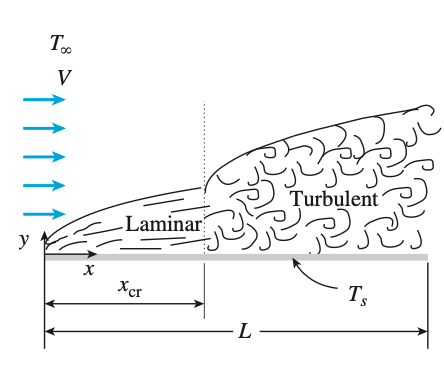
\includegraphics[width=0.5\linewidth]{./figures/flatplateflow.png}
  \caption{Laminar and turbulent flowregions of the boundary layer during flow over a flat plate. Reproduced from \citepage{cengel2015heatmasstransfer}{Fig.~7--6}.}
  \label{fig:flatplateflow}
\end{figure}

\subsubsection{Friction Coefficient}
For laminar flow over a plate the boundary layer coefficient is analytically determined to be \citepage{cengel2015heatmasstransfer}{Eq.~(7--12a, b)}:
\begin{equation} \label{eq:laminarfriction}
  \delta = \frac{\num{4,91} x}{\sqrt{\mathrm{Re}_x}}, \quad C_{f,x} = \frac{\num{0,664} }{\sqrt{\mathrm{Re}_x}}, \quad \mathrm{Re}_x < \num{5e5} 
.\end{equation}
From experiments the corresponding relations for turbulent flow are found to be \citepage{cengel2015heatmasstransfer}{Eq.~(7--13a, b)}
\begin{equation} \label{eq:turbulentfriction}
  \delta = \frac{\num{0,38} x}{\sqrt[5]{\mathrm{Re}_x}}, \quad C_{f,x} = \frac{\num{0,059} }{\sqrt[5]{\mathrm{Re}_x}}, \quad \num{5e5} \leq \mathrm{Re}_x \leq \num{e7}
.\end{equation}
Note the local friction coefficient $C_{f,x} \propto \mathrm{Re}_x^{- 1 / 2}$ and thus to $x^{- 1 / 2}$ for laminar flow.
Hence, $C_{f,x}$ is supposedly infinite at the leading edge and decreases by a factor of $x^{- 1 / 2}$ in the flow direction.
Also, note that $C_{f,x}$ reaches its highest value when the flow turns fully turbulent, where after it decreases by a factor of $x^{- 1 / 5}$ in the flow direction.

The average friction coefficient over the entire surface is then found using integration over the entire length \citepage{cengel2015heatmasstransfer}{Eq.~(7--7)}
\begin{equation} \label{eq:avgfriction}
  C_f = \frac{1}{L} \int_{0}^{L} C_{f,x} \, \mathrm{d}x
.\end{equation}
Substituting \mref{eq:laminarfriction} and \mref{eq:turbulentfriction} into \mref{eq:avgfriction} and performing the integration we obtain \citepage{cengel2015heatmasstransfer}{Eqs.~(7--14)--(7--15)}
\begin{align}
  \text{Laminar:}& & C_f &= \frac{\num{1,33}}{\sqrt{\mathrm{Re}_L}}, & \mathrm{Re}_L &< \num{5e5}  \label{eq:laminarfrictioncoeff} \\
  \text{Turbulent:}& & C_f &= \frac{\num{0,074}}{\sqrt[5]{\mathrm{Re}_L}}, & \num{5e5} \leq \mathrm{Re}_L &\leq \num{e7} \label{eq:turbulentfrictioncoeff}
.\end{align}
\Mref{eq:laminarfrictioncoeff} gives the average friction coefficient for the entire plate when the flow is laminar over the entire plate, note that this is twice the value of the local friction coefficient at the end of the plate, $C_f = 2 C_{f,x=L}$.
\Mref{eq:turbulentfrictioncoeff} gives the average friction over the entire plate when the flow is turbulent over the entire plate or when the laminar flow region is small enough to be neglected $x_{\mathrm{cr}} \ll L$.

To obtain the actual friction coefficient over a plate with both a laminar and turbulent region, the integration in \mref{eq:avgfriction} is carried out over the laminar region using \mref{eq:laminarfriction} and the turbulent region using \mref{eq:turbulentfriction} as \citepage{cengel2015heatmasstransfer}{Eq.~(7--16)}
\begin{equation} \label{eq:frictioncoeffplate}
  C_f = \frac{1}{L} \left( \int_{0}^{x_{\mathrm{cr}}} C_{f,x, \text{laminar}} \, \mathrm{d}x  + \int_{x_{\mathrm{cr}}}^{L} C_{f, x, \text{turbulent}} \, \mathrm{d}x  \right)
.\end{equation}
Taking the critical Reynolds number to be $\mathrm{Re}_{\mathrm{cr}} = \num{5e5}$ the integration in \mref{eq:frictioncoeffplate} is solved to obtain the following expression for the average friction coefficient over the entire plate
\begin{equation} \label{eq:frictioncoeffplatesimplified}
  C_f = \frac{\num{0,074} }{\sqrt[5]{\mathrm{Re}_L}} - \frac{1742}{\mathrm{Re}_L}, \quad \num{5e5} \leq \mathrm{Re}_L \leq \num{e7} 
.\end{equation}
In \mref{eq:frictioncoeffplatesimplified} the surfaces are assumed to be smooth and the free stream is assumed turbulence tree.

For laminar flow, the friction coefficient only depends on Reynolds number, whereas for turbulent flow, surface roughness causes the friction coefficient to increase many times.
Experimental observations give a average friction coefficient for turbulent flow over rough surfaces as:
\begin{equation*}
  C_f = \left( \num{1,89} - \num{1,62} \log \frac{\epsilon}{L} \right)^{-\num{2,5}}
,\end{equation*}
where $\epsilon$ is the surface roughness and $L$ is the length of the plate in the flow direction.
This relation is applicable for turbulent flow on rough surfaces for $\mathrm{Re} > \num{e6}$ especially when $\epsilon / L > \num{e-4}$ \citepage{cengel2015heatmasstransfer}{429--430}.

\subsubsection{Heat Transfer Coefficient}
The locals Nusselt number at a location $x$ for laminar flow over a flat plate can be found analytically by solving the differential energy equation to be \citepage{cengel2015heatmasstransfer}{Eq.~(7--19)}
\begin{equation*}
  \mathrm{Nu}_x = \frac{h_x x}{k} = \num{0,332} \sqrt{\mathrm{Re}_x} \sqrt[3]{\mathrm{Pr}}, \quad \mathrm{Pr} > \num{0,6}, \mathrm{Re}_x < \num{5e5}.
.\end{equation*}
From experiments, the corresponding relation for turbulent flow is \citepage{cengel2015heatmasstransfer}{Eq.~(7--20)}
\begin{equation*}
  \mathrm{Nu}_x = \frac{h_x x}{k} = \num{0,0296} \mathrm{Re}_x^{\num{0,8}} \sqrt[3]{\mathrm{Pr}}, \quad \num{0,6} \leq \mathrm{Pr} \leq \num{60}, \num{5e5} \leq \mathrm{Re}_x \leq \num{e7}
.\end{equation*}
Like, for the friction coefficient $h_x$ is, for laminar flow, proportional to $\sqrt{\mathrm{Re}_x}$ and thus to $x^{-1 / 2}$, meaning $h_x$ is supposedly infinite at the leading edge and decreases by a factor of $x^{- 1 / 2}$ in the flow direction.

Like for the friction coefficient the average convection coefficient over the entire surface is found through integration \citepage{cengel2015heatmasstransfer}{Eq.~(7--8)}
\begin{equation*}
  h = \frac{1}{L} \int_{0}^{L} h_x \, \mathrm{d}x 
.\end{equation*}
Hence, the average Nusselt number over the entire plate is \citepage{cengel2015heatmasstransfer}{Eqs.~(7--21)--(7--22)}
\begin{align}
  \text{Laminar:}& & \mathrm{Nu} &= \frac{h L}{k} = \num{0,664} \sqrt{\mathrm{Re}_L} \sqrt[3]{\mathrm{Pr}}, & \mathrm{Re}_L < \num{5e5}&, \mathrm{Pr} > \num{0,6}    \\
  \text{Turbulent:}& & \mathrm{Nu} &= \frac{h L}{k} = \num{0,037} \mathrm{Re}_L^{\num{0,8} } \sqrt[3]{\mathrm{Pr}}, & \num{5e5} \leq \mathrm{Re}_L \leq \num{e7}&, \num{0,6} \leq \mathrm{Pr} \leq \num{60} 
.\end{align}
Here, the same conditions apply as for the friction coefficient in that the laminar result only applies for fully laminar flow and vice versa for the turbulent result.
An accurate heat transfer coefficient can be found by performing the same integration as for the friction coefficient.
Taking the critical Reynolds number to be $\mathrm{Re}_{\mathrm{cr}} = \num{5e5} $ the resulting average Nusselt number over the entire plate is \citepage{cengel2015heatmasstransfer}{Eq.~(7--24)}
\begin{equation*}
  \mathrm{Nu} = \frac{h L}{k} = \left( \num{0,037} \mathrm{Re}_L^{\num{0,8} } - \num{871} \right) \sqrt[3]{\mathrm{Pr}}, \quad \num{0,6} \leq \mathrm{Pr} \leq \num{60}, \num{5e5} \leq \mathrm{Re}_L \leq \num{e7} 
.\end{equation*}
Using curve-fitting the following relation for the Nusselt number, which is claimed to be applicable for all Prandtl numbers with an accuracy of $\pm \qty{1}{\percent}$ \citepage{cengel2015heatmasstransfer}{Eq.~(7--26); pp.~430--432}
\begin{equation*}
  \mathrm{Nu}_x = \frac{h_c x}{k} = \frac{\num{0,3387} \sqrt[3]{\mathrm{Pr}} \sqrt{\mathrm{Re}_x}}{\sqrt[4]{1 + \left( \num{0,0468} / \mathrm{Pr} \right)^{2 / 3}}}, \qquad \mathrm{Re}_x \mathrm{Pr} \geq \num{100}
.\end{equation*}

\subsection{Flow Across Cylinders and Spheres}
The characteristic length for a circular cylinder or sphere is the external diameter $D$.
Thus, the Reynolds number for a circular cylinder or sphere is $\mathrm{Re} = \mathrm{Re}_D = V D / \nu$, where $V$ is the velocity as it approaches the cylinder or sphere.
The critical Reynolds number for flow across a circular cylinder or sphere is about $\mathrm{Re}_{\mathrm{cr}} \approx \num{2e5} $ \citepage{cengel2015heatmasstransfer}{438}.

\subsubsection{Heat Transfer Coefficient}
Flows across cylinders and spheres generally involve flow separation and are thus difficult to analyze analytically.
Hence, such flows much be studied experimentally or numerically.
The average Nusselt number for cross flow over a cylinder is given by \citepage{cengel2015heatmasstransfer}{Eq.~(7--35)}
\begin{equation*}
  \mathrm{Nu}_{\mathrm{cyl}} = \frac{h D}{k} = \num{0,3} + \frac{\num{0,62} \sqrt{\mathrm{Re}} \sqrt[3]{\mathrm{Pr}}}{\sqrt[4]{1 + \left( \num{0,4} / \mathrm{Pr} \right)^{2 / 3}}} \left( 1 + \left( \frac{\mathrm{Re}}{\num{282000}} \right)^{5 / 8} \right)^{4 / 5}
.\end{equation*}
For flow over a sphere, the average Nusselt number is \citepage{cengel2015heatmasstransfer}{Eq.~(7--36)}
\begin{gather*}
  \mathrm{Nu}_{\mathrm{sph}} = \frac{h D}{k} = 2 + \left( \num{0,4} \sqrt{\mathrm{Re}} + \num{0,06} \mathrm{Re}^{2 / 3} \right) \mathrm{Pr}^{\num{0,4}} \sqrt[4]{\frac{\mu_{\infty}}{\mu_s}}, \\
  \num{3,5} \leq \mathrm{Re} \leq \num{8e4}, \quad \num{0,7} \leq \mathrm{Pr} \leq \num{380}, \quad \num{1,0} \leq \mu_{\infty} / \mu_s \leq \num{3,2}
.\end{gather*}
All the fluid properties in this case are evaluated at the free-stream temperature $T_{\infty}$, except for $\mu_s$, which is evaluated at the surface temperature $T_s$.

The average Nusselt number for flow across cylinders can be expressed compactly as \citepage{cengel2015heatmasstransfer}{Eq.~(7--37)}
\begin{equation*}
  \mathrm{Nu}_{\mathrm{cyl}} = \frac{h D}{k} = C \mathrm{Re}^{m} \mathrm{Pr}^{n}
,\end{equation*}
where $n = 1 / 3$ and the experimentally determined constants $C$ and $m$ are given in \mref{tab:nusselt-crossflow-cylinders} \citepage{cengel2015heatmasstransfer}{442--443}.

\begin{table}[htbp]
  \centering
  \caption{Empirical correlations for the average Nusselt number for forced
    convection over circular and noncircular cylinders in crossflow.
    Adapted from \citepage{cengel2015heatmasstransfer}{Tab.~7--1}.}
  \label{tab:nusselt-crossflow-cylinders}
  \small
  \begin{tabularx}{\linewidth}{
    @{}
    >{\raggedright\arraybackslash}p{0.21\linewidth}
    >{\raggedright\arraybackslash}p{0.13\linewidth}
    >{\raggedright\arraybackslash}p{0.19\linewidth}
    >{\raggedright\arraybackslash}X
    @{}
  }
    \toprule
    Cross-section of cylinder & Fluid & Range of $\mathrm{Re}$ & Nusselt number \\
    \midrule

    Circle
      & Gas or liquid
      & \makecell[l]{%
        \numrange{0,4}{4} \\
        \numrange{4}{40} \\
          \numrange{40}{4000} \\
          \numrange{4000}{40000} \\
        \numrange{40000}{400000}}
      & \makecell[l]{%
          $\mathrm{Nu}=\num{0,989} \mathrm{Re}^{\num{0,330}}\mathrm{Pr}^{1/3}$\\
          $\mathrm{Nu}=\num{0,911} \mathrm{Re}^{\num{0,385} }\mathrm{Pr}^{1/3}$\\
          $\mathrm{Nu}=\num{0,683} \mathrm{Re}^{\num{0,466} }\mathrm{Pr}^{1/3}$\\
          $\mathrm{Nu}=\num{0,193} \mathrm{Re}^{\num{0,618} }\mathrm{Pr}^{1/3}$\\
          $\mathrm{Nu}=\num{0,027} \mathrm{Re}^{\num{0,805} }\mathrm{Pr}^{1/3}$}
    \\
    \midrule

    Square
      & Gas
      & \numrange{3900}{79000} 
      & $\mathrm{Nu}=\num{0,094} \mathrm{Re}^{\num{0,675} }\mathrm{Pr}^{1/3}$
    \\
    \midrule

    Square, tilted \qty{45}{\degree} 
      & Gas
      & \numrange{5600}{111000} 
      & $\mathrm{Nu}=\num{0,258} \mathrm{Re}^{\num{0,588} }\mathrm{Pr}^{1/3}$
    \\
    \midrule

    Hexagon
      & Gas
      & \numrange{4500}{90700} 
      & $\mathrm{Nu}=\num{0,148} \mathrm{Re}^{\num{0,638} }\mathrm{Pr}^{1/3}$
    \\
    \midrule

    Hexagon, tilted $45^\circ$
      & Gas
      & \makecell[l]{%
      \numrange{5200}{20400} \\
      \numrange{20400}{105000} }
      & \makecell[l]{%
          $\mathrm{Nu}=\num{0,162} \mathrm{Re}^{\num{0,638} }\mathrm{Pr}^{1/3}$\\
          $\mathrm{Nu}=\num{0,039} \mathrm{Re}^{\num{0,782} }\mathrm{Pr}^{1/3}$}
    \\
    \midrule

    Vertical plate
      & Gas
      & \numrange{6300}{23600} 
      & $\mathrm{Nu}=\num{0,257} \mathrm{Re}^{\num{0,731} }\mathrm{Pr}^{1/3}$
    \\
    \midrule

    Ellipse
      & Gas
      & \numrange{1400}{8200} 
      & $\mathrm{Nu}=\num{0,197} \mathrm{Re}^{\num{0,612} }\mathrm{Pr}^{1/3}$
    \\

    \bottomrule
  \end{tabularx}
\end{table}

\subsubsection{Flow Across Tube Banks}
Flow through tube banks is studied experimentally as it is too complex to be treated analytically.
The average Nusselt number over the entire tube bank is \citepage{cengel2015heatmasstransfer}{Eq.~(7--42)}
\begin{equation*}
  \mathrm{Nu}_D = \frac{h D}{k} C \mathrm{Re}_D^{m} \mathrm{Pr}^{n} \sqrt[4]{\mathrm{Pr} / \mathrm{Pr}_s}
,\end{equation*}
where $D$ is the tube diameter and the values of the constants $C$, $m$, and $n$ depend on the Reynolds number.
Such correlations are given in \mref{tab:nusselt-tube-banks} for tube banks with more than \num{16} rows $N_L > 16$, $\num{0,7} < \mathrm{Pr} < \num{500}$ and $0 < \mathrm{Re}_D < \num{2e6} $ with an uncertainty of $\pm \qty{15}{\percent}$.
Note that all properties except $\mathrm{Pr}_s$ are evaluated at the arithmetic mean temperature $T_m$ of the fluid determined from \citepage{cengel2015heatmasstransfer}{Eq.~(7--43)}
\begin{equation*}
  T_m = \frac{T_i + T_e}{2}
\end{equation*}
where $T_i$ and $T_e$ are the fluid inlet and exit temperatures of the tube bank respectively.

The average Nusselt number relations given in \mref{tab:nusselt-tube-banks} are only applicable for tube banks with more than \num{16} rows.
These relations can also be used for tube banks with $N_L < \num{16}$ provided they are modified using \citepage{cengel2015heatmasstransfer}{Eq.~(7--44)}
\begin{equation} \label{eq:corneeded}
  \mathrm{Nu}_{D, N_{L < \num{16} }} = F \mathrm{Nu}_D
,\end{equation}
where $F$ is a correction factor whose values are given in \mref{tab:tube-bank-correction-factor}.
For $\mathrm{Re}_D > \num{1000}$ the correction factor is independent of Reynolds number. 



\begin{table}[htbp]
  \centering
  \caption{Nusselt number correlations for crossflow over tube banks for
  $N_L > \num{16}$ and $\num{0,7}  < \mathrm{Pr} < \num{500} $. Adapted from \citepage{cengel2015heatmasstransfer}{Tab.~7--2}.}
  \label{tab:nusselt-tube-banks}
  \small
  \begin{tabularx}{\linewidth}{
    @{}
    >{\raggedright\arraybackslash}p{0.17\linewidth}
    >{\raggedright\arraybackslash}p{0.22\linewidth}
    >{\raggedright\arraybackslash}X
    @{}
  }
    \toprule
    Arrangement & Range of $\mathrm{Re}_D$ & Correlation \\
    \midrule

    \multirow{4}{*}{In-line}
                & \numrange{0}{100} 
      & $\mathrm{Nu}_D = \num{0,9}\mathrm{Re}_D^{\num{0,4} } \mathrm{Pr}^{\num{0,36} }(\mathrm{Pr}/\mathrm{Pr}_s)^{\num{0,25} }$ \\
      & \numrange{100}{1000} 
      & $\mathrm{Nu}_D = \num{0,52} \mathrm{Re}_D^{\num{0,5} } \mathrm{Pr}^{\num{0,36} }(\mathrm{Pr}/\mathrm{Pr}_s)^{\num{0,25} }$ \\
      & \numrange{1000}{2e5} 
      & $\mathrm{Nu}_D = \num{0,27} \mathrm{Re}_D^{\num{0,63} } \mathrm{Pr}^{\num{0,36} }(\mathrm{Pr}/\mathrm{Pr}_s)^{\num{0,25} }$ \\
      & \numrange{2e5}{2e6} 
      & $\mathrm{Nu}_D = \num{0,033}\mathrm{Re}_D^{\num{0,8} } \mathrm{Pr}^{\num{0,4} }(\mathrm{Pr}/\mathrm{Pr}_s)^{\num{0,25} }$ \\
    \midrule

    \multirow{4}{*}{Staggered}
      & \numrange{0}{500} 
      & $\mathrm{Nu}_D = \num{1,04}\mathrm{Re}_D^{\num{0,4} }\mathrm{Pr}^{\num{0,36} }(\mathrm{Pr}/\mathrm{Pr}_s)^{\num{0,25} }$ \\
      & \numrange{500}{1000} 
      & $\mathrm{Nu}_D = \num{0,71}\mathrm{Re}_D^{0.5} \mathrm{Pr}^{0.36}(\mathrm{Pr}/\mathrm{Pr}_s)^{0.25}$ \\
      & \numrange{1000}{2e5} 
      & $\mathrm{Nu}_D = \num{0,35} (S_T/S_L)^{\num{0,2} } \mathrm{Re}_D^{\num{0,6} }\mathrm{Pr}^{\num{0,36} } (\mathrm{Pr}/\mathrm{Pr}_s)^{\num{0,25} }$ \\
      &  \numrange{2e5}{2e6} 
      & $\mathrm{Nu}_D = \num{0,031} (S_T/S_L)^{\num{0,2} } \mathrm{Re}_D^{\num{0,8} }\mathrm{Pr}^{\num{0,36} } (\mathrm{Pr}/\mathrm{Pr}_s)^{\num{0,25} }$ \\
    \bottomrule
  \end{tabularx}
\end{table}

\begin{table}[htbp]
  \centering
  \caption{Correction factor $F$ for use in \mref{eq:corneeded} for $N_L<16$ and
    $\mathrm{Re}_D>1000$. Adapted from  \citepage{cengel2015heatmasstransfer}{Tab.~7--3}.}
  \label{tab:tube-bank-correction-factor}
  \begin{tabular}{@{}l*{8}{c}@{}}
    \toprule
    $N_L$ & \num{1}  & \num{2}  & \num{3}  & \num{4}  & \num{5}  & \num{7}  & \num{10}  & \num{13}  \\
    \midrule
    In-line   & \num{0,70}  & \num{0,80}  & \num{0,86}  & \num{0,90}  & \num{0,93}  & \num{0,96}  & \num{0,98}  & \num{0,99}  \\
    Staggered & \num{0,64}  & \num{0,76}  & \num{0,84}  & \num{0,89}  & \num{0,93}  & \num{0,96}  & \num{0,98}  & \num{0,99}  \\
    \bottomrule
  \end{tabular}
\end{table}

Once the Nusselt number and therefore the heat transfer coefficient for the entire tube bank is known, the heat transfer rate can be determined from Newton's law of cooling using a suitable temperature difference $\Delta T$.
This suitable temperature difference is, for internal flow, the log mean temperature difference $\Delta T_{1m}$ defined as \citepage{cengel2015heatmasstransfer}{Eq.~(7--45)}
\begin{equation*}
  \Delta T_{1m} = \frac{\left( T_s - T_e \right) - \left( T_s - T_i \right)}{\ln \left( \frac{T_s - T_e}{T_s - T_i} \right)} = \frac{\Delta T_e - \Delta T_i}{\ln \left( \frac{\Delta T_e}{\Delta T_i} \right)}
.\end{equation*}
Also, the exit temperature of the fluid $T_e$ can be determined from \citepage{cengel2015heatmasstransfer}{Eq.~(7--46)}
\begin{equation*}
  T_e = T_s - \left( T_s - T_i \right) \exp \left( - \frac{A_s h}{\dot{m} c_p} \right)
,\end{equation*}
where $A_s = N \pi D L$ is the heat transfer surface area and $\dot{m} = \rho V N_t S_T L$ is the mass flow rate of the fluid.
Here, $N$ is the total number of tubes in the bank, i.e. the product of $N_T$ and $N_L$ which are the number of tubes in the transverse plane and longitudinal plane respectively, $L$ is the length of the tubes, and $V$ is the velocity of the fluid just before entering the tube bank.
The heat transfer rate can be determined from \citepage{cengel2015heatmasstransfer}{Eq.~(7--47)}
\begin{equation*}
  \dot{Q} = h A_s \Delta T_{1m} = \dot{m} c_p \left( T_e - T_i \right)
.\end{equation*}
In the above the second relation is usually more convenient as it does not require the calculation of $\Delta T_{1m}$ \citepage{cengel2015heatmasstransfer}{446--449}.

% !TeX root = ../master.tex

\lecture{7}{2026-10-13}{Convection, Pt. III}


% WORKFLOW:LECTURES-END

\printbibliography

\end{document}
